% настойка языка и шрифта
\documentclass[12pt]{article} 
%\usepackage[utf8]{inputenc}
%\DeclareUnicodeCharacter{00A0}{ }
%\DeclareUnicodeCharacter{2212}{-}

\usepackage[utf8]{inputenc}
\usepackage[T2A]{fontenc}
\usepackage[english,russian]{babel}



\usepackage{cmap}
\usepackage[russian]{babel}

% настройка страниц
\usepackage[left=3cm, right=1.5cm, top=2cm, bottom =2cm]{geometry}
\geometry{a4paper} 

% дополнительные пакеты
\usepackage{array}
\usepackage{float}
\usepackage{amsmath} 
\usepackage{indentfirst}
\usepackage{textalpha}
\usepackage{mathtext}
\usepackage[pdftex]{graphicx}
\usepackage{csquotes} 
\graphicspath{{img/}} %путь к рисункам
\DeclareGraphicsExtensions{.pdf,.png,.jpg}

%переносы в таблицах
\newcommand{\specialcell}[2][c]{%
	\begin{tabular}[#1]{@{}c@{}}#2\end{tabular}}

\usepackage[
bookmarks=true, colorlinks=true, unicode=true,
urlcolor=black,linkcolor=black, anchorcolor=black,
citecolor=black, menucolor=black, filecolor=black,
]{hyperref}


\usepackage{enumerate} %списки
\setcounter{page}{2} 
\addto\captionsrussian{\def\refname{}} %заголовок библиографии

\usepackage{natbib}
\usepackage{pgfplots}
\usepackage{listings} %% собственно, это и есть пакет listings
\usepackage{caption}
%% код ниже нарисует серую рамочку вокруг заголовка кода.
\DeclareCaptionFormat{listing}{\colorbox{white}{\parbox{\textwidth}{#1#2#3}}}
\captionsetup[lstlisting]{format=listing,labelfont=black,textfont=black}

\begin{document}
\lstset{ %
language=C,                 % выбор языка для подсветки
basicstyle=\small\sffamily, % размер и начертание шрифта для подсветки кода
numbers=left,               % где поставить нумерацию строк (слева\справа)
numberstyle=\tiny,           % размер шрифта для номеров строк
stepnumber=1,                   % размер шага между двумя номерами строк
numbersep=5pt,                % как далеко отстоят номера строк от подсвечиваемого кода
backgroundcolor=\color{white}, % цвет фона подсветки - используем \usepackage{color}
showspaces=false,            % показывать или нет пробелы специальными отступами
showstringspaces=false,      % показывать или нет пробелы в строках
showtabs=false,             % показывать или нет табуляцию в строках
frame=false,              % рисовать рамку вокруг кода
tabsize=1,                 % размер табуляции по умолчанию равен 2 пробелам
captionpos=t,              % позиция заголовка вверху [t] или внизу [b] 
breaklines=true,           % автоматически переносить строки (да\нет)
breakatwhitespace=false, % переносить строки только если есть пробел
escapeinside={\%*}{*)},  % если нужно добавить комментарии в коде
extendedchars=\true
}

%обложка
\begin{center}
	\hfill \break
	\textit{
		\normalsize {\bf  Министерство науки и высшего образования Российской Федерации}\\
		\normalsize {\bf Федеральное государственное бюджетное образовательное учреждение }\\
		\normalsize {\bf  высшего  образования}
		\normalsize  {\bf  «Московский государственный технический университет}\\ 
		\normalsize  {\bf имени Н. Э. Баумана}\\
		\normalsize  {\bf (национальный исследовательский университет)»}\\
		\normalsize  {\bf (МГТУ им. Н.Э. Баумана)}\\
	}
	\noindent\rule{\textwidth}{2pt}
	\hfill \break
	\hfill\break
	\hfill\break
	\hfill\break
	\hfill\break
	\hfill\break
	\hfill\break
	\hfill \break
	\hfill \break
	\textit{
		\normalsize {\bf РАСЧЕТНО-ПОЯСНИТЕЛЬНАЯ ЗАПИСКА}\\
		\normalsize {\bf к курсовому проекту на тему:}\\
		\normalsize {\bf  Поиск фильмов по параметрам и просмотр информации о них} \\
	}
	\hfill \break
	\hfill \break
	\hfill \break
	\hfill \break
	\hfill \break
	\hfill \break
	\hfill \break
	\hfill \break
	\hfill \break
	\hfill \break
	\hfill \break
	
	\hfill \break
	\normalsize {
		\noindent
		\makebox[0pt][l]{Студент}%
		\makebox[\textwidth][c]{}%
		\makebox[0pt][r]{{$\underset{\text{(Подпись, дата)}}{\underline{\hspace{4cm}}}$ \space 
		Полякова К. А.}}
	}\\
	\hfill \break
	\hfill \break
	\normalsize {
		\noindent
		\makebox[0pt][l]{Руководитель курсового проекта}%
		\makebox[\textwidth][c]{}%
		\makebox[0pt][r]{{$\underset{\text{(Подпись, дата)}}{\underline{\hspace{5cm}}}$ \space 
		Филиппов М. В.}}
	}
	\hfill \break
	\hfill \break
	\hfill \break
	\hfill \break\hfill \break
	\hfill \break
\end{center}
\hfill \break
\hfill \break
\begin{center} Москва 2020\end{center}

\thispagestyle{empty} 
\tableofcontents
\newpage
\section*{Введение}
\addcontentsline{toc}{section}{Введение}

Еще пару десятков лет назад, чтобы посмотреть какой-либо фильм люди посещали кинотеатры или смотреть телевизор. Но тогда выбор был очень ограниченный - приходилось смотреть только то, что шло в кинотеатрах или показывали по телевизору.

Современный же человек не имеет таких ограничений. С появлением Интернета огромное количество различных фильмов, сериалов, мультфильмов доступны каждому прямо из дома. Необходимо заметить, что и количество кинофильмов увеличилось в несколько раз. Как же не запутаться в таком многообразии и выбрать именно то, что нравится? Именно для этого необходимы приложения для поиска по различным параметрам и для просмотра необходимой информации, чтобы найти именно то, что понравится.
\hfill \break

Целью данной курсовой работы является создание клиент–серверного приложения <<Хочу посмотреть!>>, которое предоставляет доступ к фильмам и возможность просмотра информации о них. Также пользователь может добавить любые фильмы в "Избранное" для того, чтобы посмотреть их позже или пересмотреть. В приложении можно осуществить поиск по нескольким параметрам: по названию, по году премьеры, по стране или по жанру.

Актуальность разработки состоит в том, что с помощью такого приложения можно с легкостью найти информацию о фильме или добавить фильм в "Избранное", чтобы не забыть его посмотреть.

Для выполнения цели необходимо выполнить следующие задачи:
\begin{itemize}
	\item формализовать задачу в виде определения необходимого функционала;
	\item провести анализ существующих СУБД;
	\item спроектировать базу данных, необходимую для хранения и структурирования данных;
	\item реализовать спроектированную базу данных с использованием выбранной СУБД;
	\item реализовать приложение для взаимодействия с реализованной БД.
\end{itemize}

\newpage
\section{Аналитическая часть}%
\setcounter{section}{1}

В данном разделе будут рассмотрены общие сведения о БД и СУБД, типы БД и используемые framework. 

\subsection{Формализация задачи}%
\setcounter{subsection}{1}

В соответствии с техническим заданием на курсовой проект пользователям необходма система авторизации и регистрации для предоставления индивидуальной информации.

Также должна быть предусмотрена возможность поиска и просмотра информации о фильмах, а также добавление и удаление фильмов из "Избранного".


\subsection{Общие сведения о БД  СУБД}%
\setcounter{subsection}{2}
База данных представляет собой совокупность определенным образом организованных данных, которые хранятся в памяти вычислительной системы и отображают состояние объектов и их взаимосвязи в рассматриваемой предметной области.\\
Под системой управления базами данных \(СУБД\) понимается совокупность программных и языковых средств, предназначенных для создания и обработки БД. 

\subsection{Типы БД}
\setcounter{subsection}{3}

Модель данных определяет логическую структуру БД и то, каким образом данные будут храниться, организовываться и обрабатываться. 

Существует 3 типа моделей организации данных:
\begin{itemize}
	\item иерархическая модель БД;
	\item сетевая модель БД;
	\item реляционная модель.
\end{itemize}

\subsubsection{Иерархическая модель БД}
\setcounter{subsubsection}{1}

Иерархическая модель БД представляет собой древовидную (иерархическую) структуру, состоящую из объектов (данных) различных уровней. Каждый объект может включать в себя несколько объектов более низкого уровня. Такие объекты находятся в отношении предка (объект более близкий к корню) к потомку (объект более низкого уровня), при этом возможна ситуация, когда объект-предок имеет несколько потомков, тогда как у объекта-потомка обязателен только один предок.

Иерархической базой данных является файловая система, состоящая из корневого каталога, в котором имеется иерархия подкаталогов и файлов.

Связи записей реализуются в виде физических указателей с одной записи на другую. Основной недостаток иерархической структуры – невозможность реализовать отношения "многие-ко-многим", а также ситуации, в которых запись имеет несколько предков. \cite{0}

\begin{figure}[h]
	\center{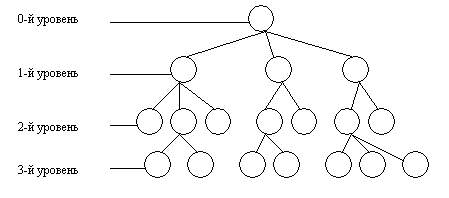
\includegraphics[scale=0.6]{1.jpg}}
	\caption{Иерархическая модель БД}
	\label{fig:image}
\end{figure}

\subsubsection{Сетевая модель}
\setcounter{subsubsection}{2}

Сетевая модель данных является расширением иерархического подхода. 
Разница между иерархической моделью данных и сетевой заключается в том, что в иерархических структурах запись-потомок должна иметь в точности одного предка, а в сетевой структуре у потомка может быть любое число предков. 
Записи в такой модели связаны списками с указателями.

Примером сетевой СУБД является IDMS (интегрированная система управления данными) от компании Computer Associates international Inc.

Популярность сетевой модели совпала с популярностью иерархической модели. 
Некоторые данные намного естественнее моделировать с несколькими предками для одного дочернего элемента. 
Сетевая модель позволяла моделировать отношения «многие-ко-многим».

И хотя эта модель широко применялась на практике, она так и не стала доминантной по двум основным причинам. 
Во-первых, компания IBM решила не отказываться от иерархической модели в расширениях для своих продуктов, таких как IMS и DL/I. 
Во-вторых, через некоторое время ее сменила реляционная модель, предлагавшая более высокоуровневый, декларативный интерфейс. \cite{0}

\begin{figure}[h]
	\center{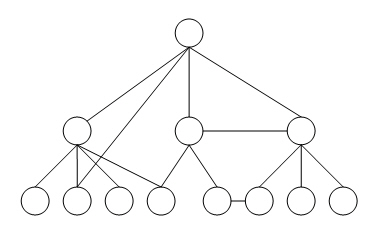
\includegraphics[scale=0.6]{2.jpg}}
	\caption{Сетевая модель БД}
	\label{fig:image}
\end{figure}

\subsubsection{Реляционная модель}
\setcounter{subsubsection}{3}

В реляционной модели, в отличие от иерархической или сетевой, не существует физических отношений. Вся информация хранится в виде таблиц (отношений), состоящих из рядов и столбцов. А данные двух таблиц связаны общими столбцами, а не физическими ссылками или указателями. Объекты и их отношения представлены таблицами.

В реляционных моделях нет необходимости просматривать все указатели, что облегчает выполнение запросов на выборку информации по сравнению с сетевыми и иерархическими БД. Это одна из основных причин, почему реляционная модель оказалась более удобна.

Распространенные реляционные СУБД: MySql, PostgreSql, Access, Oracle, DB2, MS-SQL Server, SQLite.
Каждая реляционная таблица представляет собой двумерный массив и обладает следующими свойствами:

\begin{itemize}
	\item каждый элемент таблицы — один элемент данных;
	\item все элементы в одном столбце имеют одинаковый тип;
	\item каждый столбец имеет уникальное имя;
	\item одинаковые строки (записи, кортежи) в таблице отсутствуют;
	\item порядок следования строк и столбцов может быть произвольным.
\end{itemize}

Каждое поле содержит одну характеристику объекта предметной области. В записи собраны сведения об одном экземпляре этого объекта.

Некоторые поля могут быть определены как ключевые. Это значит, что для ускорения поиска конкретных значений будет использоваться индексация. Когда поля двух различных таблиц получают данные из одного набора, можно использовать оператор JOIN для выбора связанных записей двух таблиц, сопоставив значения полей. Такие действия можно расширить до объединения нескольких полей в нескольких таблицах. Поскольку отношения здесь определяются только временем поиска, реляционные базы данных классифицируются как динамические системы. 

\subsubsection{Сравнение моделей}
\setcounter{subsubsection}{4}

Иерархическая модель данных поддерживает отношения типа «один-к-одному» или «один-ко-многим». Она позволяет быстро получать данные, но не отличается гибкостью. Иногда роль элемента (родителя или потомка) неясна и не подходит для иерархической модели.

Вторая, сетевая модель данных, имеет более гибкую структуру, чем иерархическая, и поддерживает отношение «многие ко многим». Но быстро становится слишком сложной и неудобной для управления.

Третья модель – реляционная – более гибкая, чем иерархическая и проще для управления, чем сетевая. Реляционная модель сегодня используется чаще всего, так как имеет множество преимуществ, таких как:

\begin{itemize}
	\item простота использования;
	\item гибкость;
	\item независимость данных;
	\item безопасность;
	\item простота практического применения;
	\item слияние данных;
	\item целостность данных.
\end{itemize}

В связи с этим далее будет рассматриваться реляционная модель. Теперь необходимо рассмотреть систему управления такой моделью.

\subsection{СУБД}%
\setcounter{subsection}{4}

Самых популярные системы управления реляционными базами данных:
\begin{itemize}
	\item MySQL;
	\item PostgreSQL; 
	\item SQLite.
\end{itemize}

В данном проекте будет рассмотрена СУБД SQLite.

Это компактная встраиваемая СУБД. Слово «встраиваемый» (embedded) означает, что SQLite не использует парадигму клиент-сервер, то есть движок SQLite не является отдельно работающим процессом, с которым взаимодействует программа, а представляет собой библиотеку, компонующуюся с программой, и движок становится составной частью программы. Таким образом, в качестве протокола обмена используются вызовы функций (API) библиотеки SQLite. Такой подход уменьшает накладные расходы, время отклика и упрощает программу.

Однако SqLite популярна скорее в случаях, когда не требуется выносить базу данных на отдельную машину и данные требуется хранить в рамках одной ОС. Будучи файловой БД, она предоставляет отличный набор инструментов для более простой (в сравнении с серверными БД) обработки любых видов данных. \cite{1}

Преимущества:

\begin{itemize}
	\item {\bf Файловая.} Вся БД хранится в одном файле, что облегчает перемещение.
	\item {\bf Стандартизированная.} SQLite использует SQL, некоторые функции не используются (RIGHT OUTER JOIN или FOR EACH STATEMENT);
	\item {\bf Отсутствие пользовательского.} Продвинутые БД предоставляют пользователям возможность управлять связями в таблицах в соответствии с привилегиями, но у SQLite такой функции нет.
	\item {\bf Невозможность дополнительной настройки.} SQLite нельзя сделать более производительной, путем изменения настроек.
\end{itemize}

\subsection{Framework}%
\setcounter{subsection}{5}

SQLite совместима со множеством фреймворков, которые содержат в себе требуемые методы обращения к БД. Среди возможных вариантов для использования в проекте были выбраны библиотеки sqlite и SQLAlchemy \cite{2}.

SQLAlchemy — это программная библиотека на языке Python для работы с реляционными СУБД с применением технологии ORM. Служит для синхронизации объектов Python и записей реляционной базы данных.

В качестве web-framework был выбран Django, который предоставляет все необходимые инструменты для создания подобного проекта, так как предоставляет возможность для написания как frontend, так и backend для полноценного запуска приложения.

\subsection{Вывод}%
\setcounter{subsection}{6}

В результате проведенного анализа в качестве модели данных была выбрана реляционная модель, в качестве СУБД – SQLite.

Таким образом, подобрав необходимый набор инструментов для реализации web-приложения, можно приступить к проектированию решения поставленной задачи.

%%%%%%%%%%%%%%%%%%%%%%%%%%%%%%%%%%%%%%%%%%%%%%%%%%%%%%%%%%%%%%%%%%%%%

\newpage
\section{Конструкторская часть}%
\setcounter{section}{2}

В соответствии с техническим заданием и аналитическим разделом должно быть получено полноценное приложение для взаимодействия с БД.

\subsection{Проектирование таблиц базы данных}%
\setcounter{subsection}{1}

База данных приложения <<ХочуПосмотреть!>> состоит из следующих таблиц:
\begin{itemize}
	\item таблица пользователей сайта {\bf User};
	\item таблица фильмов {\bf Book};
	\item таблица актеров {\bf Location};
	\item таблица режиссеров {\bf Direcor};
	\item таблица состояния книги относительно каждого пользователя {\bf Status}.
\end{itemize}

\hfill \break

{\bf Таблица User}

Позволяет однозначно идентифицировать пользователя сайта, реализовать авторизацию пользователя. Имеет связь <<один-ко-многим>> с таблицей Status. 


Таблица содержит следующие поля:
\begin{itemize}
	\item id - целочисленное поле, идентификационный номер клиента;
	\item username - символьное поле, название аккаунта;
	\item email - символьное поле, адрес электронной почты клиента;
	\item password hash - символьное поле, хэш пароля пользователя;
	\item about\_me - символьное поле, информация о пользователе;
	\item last\_seen - поле даты, время последнего посещения пользователя;
	\item image - текстовое поле, хранит аватар пользователя в формате base64.
\end{itemize}

\hfill \break

{\bf Таблица Status}

Хранит данные о статусе книги относительно пользователя. Связана с таблицами книг Book и пользователей User связью <<один-к-одному>>.

Таблица содержит следующие поля:
\begin{itemize}
	\item user\_id - целочисленное поле, идентификатор пользователя;
	\item book\_id - целочисленное поле, идентификатор книги;
	\item status - целочисленное поле, состояние книги по отношению к пользователю.
\end{itemize}

\hfill \break

{\bf Таблица Book}

В данной таблице хранятся данные о книгах. Эта таблица связана с таблицами местоположения книг Location и таблицей статуса Status связью <<один-к-одному>>.

Таблица содержит следующие поля:
\begin{itemize}
	\item id – целочисленное поле, идентификатор книги;
	\item title – символьное поле, название книги;
	\item about\_book – символьное поле, информация о книге;
	\item author – символьное поле, имя автора;
	\item image – текстовое поле, хранящее изображение книги.
\end{itemize}

\hfill \break

{\bf Таблица Location}

Таблица, содержащая информацию о расположении книг в библиотеке. С помощью связи <<один-к-одному>> связана с таблицей книг Book.

Таблица содержит следующие поля:
\begin{itemize}
	\item id – целочисленное поле, идентификатор локации;
	\item shelving – целочисленное поле, номер стеллажа;
	\item shelf – целочисленное поле, номер полки;
	\item column – целочисленное поле, номер ряда;
	\item position – целочисленное поле, номер позиции в ряду;
	\item book\_id – целочисленное поле, идентификатор книги.
\end{itemize}

\begin{figure}[h]
	\center{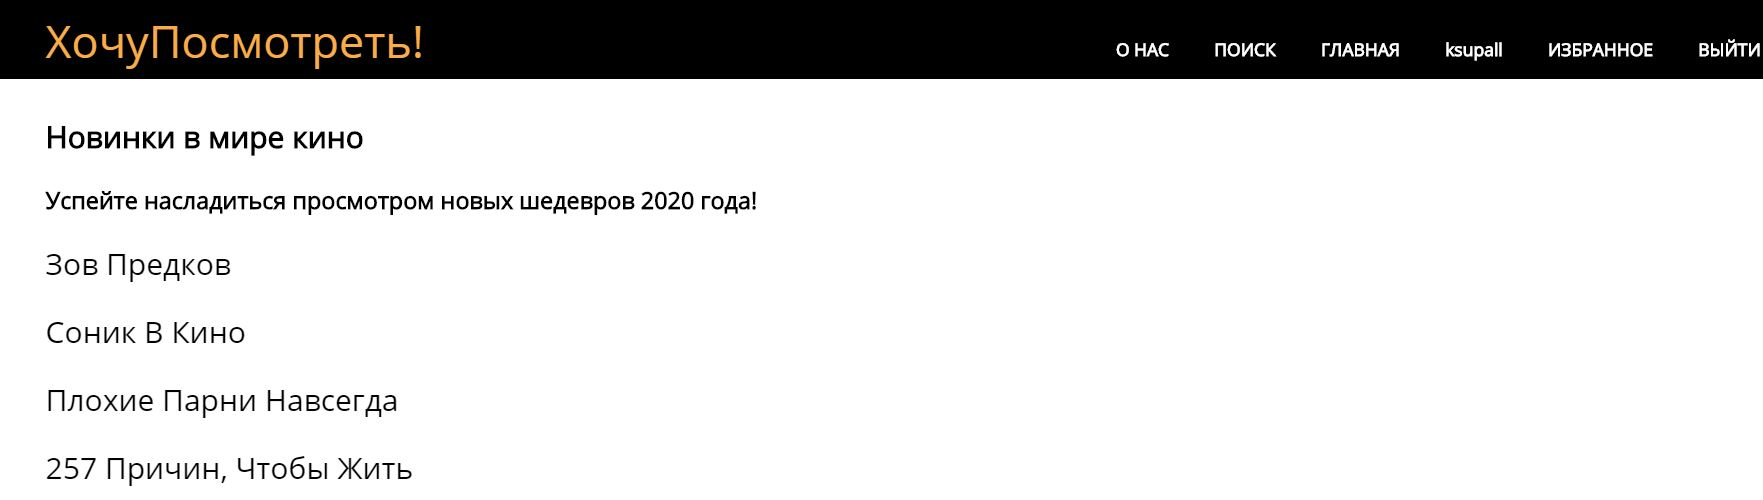
\includegraphics[scale=0.3]{8.jpg}}
	\caption{Диаграмма БД}
	\label{fig:image}
\end{figure}


\subsection{Проектирование системы изменения данных}%
\setcounter{subsection}{2}

Во Flask каждую таблицу представляет класс. Он отображает информацию о данных сущности. Он содержит поля и поведение данных. 
С помощью методов класса осуществляются операции добавления, удаления и обновления записей.

\subsection{Проектирование регистрации и аутентификации пользователя}%
\setcounter{subsection}{3}

Регистрация пользователя в приложении является добавлением в базу данных (в таблицу User) записи, содержащей необходимую информацию для аутентификации. Для этого пользователь вводит соответствующие данные  в поля регистрационной формы.

Framework Flask предоставляет собой набор данных базовых инструментов для реализации web-приложения. В этот функционал включена реализация аутентификации пользователя.


\subsection{Вывод}%
\setcounter{subsection}{4}

Была разработана модель приложения, дающего возможность вести учет книг, реализующего регистрацию, аутентификацию и авторизацию пользователей.

%%%%%%%%%%%%%%%%%%%%%%%%%%%%%%%%%%%%%%%%%%%%%%%%%%%%%%%%%%%%%%%%%%%%%

\newpage
\section{Технологическая часть}%
\setcounter{section}{3}

После проектирования структуры поставленной задачи, требуется реализовать набор функций, необходимый для создания web-приложения, а также конкретизировать полный список инструментов, используемых для запуска приложения.

\subsection{Выбор инструментов разработки}%
\setcounter{subsection}{1}

В ходе реализации были использованы следующие технологии и средства:

\begin{itemize}
	\item язык программирования Python;
	\item СУБД SQLite;
	\item библиотека Flask.
\end{itemize}

Такой набор инструментов был выбран, потому что для каждого из элементов предусмотрено взаимодействие с другими.
Также данные инструменты полностью выполняют задачи, необходимые для реализации проекта.

Использован компьютер с операционной системой macOS Mojave.

\subsection{Реализация хранения данных}%
\setcounter{subsection}{2}

Для работы с базой данных требуется объявить классы таблиц БД.

\begin{lstlisting}[label=some-code, caption=Класс <<Пользователи>>]
class User(UserMixin, db.Model):
id = db.Column(db.Integer, primary_key = True)
username = db.Column(db.String(64), index = True, unique = True)
email = db.Column(db.String(128), index = True, unique = True)
password_hash = db.Column(db.String(128))
about_me = db.Column(db.String(150))
last_seen = db.Column(db.DateTime, default = datetime.utcnow)
image = db.Column(db.Text)

book = db.relationship('Book', secondary='status', backref='users', lazy='dynamic')

def __repr__(self):
return '<User {}>'.format(self.username)

def set_password(self, password):
self.password_hash = generate_password_hash(password)

def check_password(self, password):
return check_password_hash(self.password_hash, password)

def avatar(self, size):
digest = md5(self.email.lower().encode('utf-8')).hexdigest()
return 'http://www.gravatar.com/avatar/{}?d=identicon&s={}'.format(digest, size)


def get_reset_password_token(self, expires_in=600):
return jwt.encode({'reset_password': self.id, 'exp': time() + expires_in},
app.config['SECRET_KEY'], algorithm='HS256').decode('utf-8')

def get_book(id):
conn = sqlite3.connect("app.db")
cursor = conn.cursor()
cursor.execute("select title, author, image from book where id = %d", id)
res = cursor.fetchall()
print(res)
return res

def get_books(self):
conn = sqlite3.connect("app.db")
cursor = conn.cursor()
cursor.execute("select author, title, username, book.image, book.id from (user left outer join status on user.id == status.user_id) as us \
join book on us.book_id == book.id \
where us.id = (?)", (current_user.id, ))
res = cursor.fetchall()
return res

def get_books_count(self):
conn = sqlite3.connect("app.db")
cursor = conn.cursor()
cursor.execute("select count(book.id) from (user left outer join status on user.id == status.user_id) as us \
join book on us.book_id == book.id\
where us.id = (?)", (current_user.id, ))
res = cursor.fetchall()
return res[0][0]
\end{lstlisting}

\begin{lstlisting}[label=some-code, caption=Класс <<Книги>>]
class Book(db.Model):
#__searchable__ = ['title']
id = db.Column(db.Integer, primary_key = True)
title = db.Column(db.String(60), index = True)
about_book = db.Column(db.String(150))
author = db.Column(db.String(60), index = True)
location = db.relationship('Location', uselist=False, backref='books')
image = db.Column(db.Text)

user = db.relationship(
'User', secondary='status',
backref='books', lazy='dynamic')

def __repr__(self):
return '<Book {}>'.format(self.image)

def get_book(self, id):
conn = sqlite3.connect("app.db")
cursor = conn.cursor()
cursor.execute("select title, author, image from book where id = %d", id)
res = cursor.fetchall()
print(res)
return res

def search_title(search):
conn = sqlite3.connect("app.db")
cursor = conn.cursor()
cursor.execute("select id, title, author, image from book where title like (?) ", (search, ))
res = cursor.fetchall()
conn.close()
return res

def search_author(search):
conn = sqlite3.connect("app.db")
cursor = conn.cursor()
cursor.execute("select id, title, author, image from book where author like (?) ", (search, ))
res = cursor.fetchall()
conn.close()
return res

def no_search(search):
conn = sqlite3.connect("app.db")
cursor = conn.cursor()
cursor.execute("select id, title, author, image from book where author like (?) or title like (?)", (search, search))
res = cursor.fetchall()
conn.close()
return res

def other_books_author(bookid):
conn = sqlite3.connect("app.db")
cursor = conn.cursor()
cursor.execute("select book.id, book.title, book.author, book.image, B.title, B.author, B.about_book, B.image, B.shelving, B.shelf, B.column, B.position, B.id " +
"from ( " +
"select book.id, title, author, about_book, image, shelving, shelf, column, position " +
"from book left join location on book.id = location.book_id  where book.id = (?) " +
") as B left join book on book.author = B.author and B.id != book.id;", (bookid, ))
res = cursor.fetchall()
conn.close()
return res

def get_status_book(bookid):
conn = sqlite3.connect("app.db")
cursor = conn.cursor()
cursor.execute("select status " +
"from ( " +
"select username, book.id, status " +
"from (user join status on user.id == status.user_id) as us " +
"join book on us.book_id == book.id" +
") as res where res.id = (?)", (bookid, ))
res = cursor.fetchone()
conn.close()
return res

def delete_book(book_id):
conn = sqlite3.connect("app.db")
cursor = conn.cursor()
cursor.execute("delete from status where user_id = (?) and book_id = (?)", (current_user.id, book_id))
conn.commit()
cursor.execute("delete from location where book_id = (?)", (book_id, ))
conn.commit()
cursor.execute("delete from book where id = (?)", (book_id, ))
conn.commit()
conn.close()
\end{lstlisting}

\begin{lstlisting}[label=some-code, caption=Класс <<Статус>>]
class Status(db.Model):
__tablename__ = 'status'
__table_args__ = (
PrimaryKeyConstraint('user_id', 'book_id'),
)

user_id = db.Column(db.Integer, db.ForeignKey('user.id'))
book_id = db.Column(db.Integer, db.ForeignKey('book.id'))
status = db.Column(db.Integer)

def set_status(status, book_id, username):
conn = sqlite3.connect("app.db")
cursor = conn.cursor()
cursor.execute("update status set status = (?) " +
"where book_id = (?) and user_id = (?)", (status, book_id, current_user.id))
conn.commit()
conn.close()

def join_book(book_id, status):
conn = sqlite3.connect("app.db")
cursor = conn.cursor()
cursor.execute("INSERT INTO status VALUES ((?), (?), (?))", (current_user.id, book_id, status))
conn.commit()
conn.close()

def delete_status(book_id):
conn = sqlite3.connect("app.db")
cursor = conn.cursor()
cursor.execute("delete from status where user_id = (?) and book_id = (?)", (current_user.id, book_id))
conn.commit()
conn.close()

\end{lstlisting}

\begin{lstlisting}[label=some-code, caption=Класс <<Локация>>]
class Location(db.Model):
id = db.Column(db.Integer, primary_key=True)
shelving = db.Column(db.Integer, index=True)
shelf = db.Column(db.Integer, index=True)
column = db.Column(db.Integer, index=True)
position = db.Column(db.Integer, index=True)
book_id = db.Column(db.Integer, db.ForeignKey('book.id'))

def update_location(shelving, shelf, column, position, bookid):
conn = sqlite3.connect("app.db")
cursor = conn.cursor()
cursor.execute("UPDATE location SET shelving = (?), shelf = (?), column = (?), position = (?) WHERE id = (?)", (shelving, shelf, column, position, bookid))
conn.commit()
conn.close()
\end{lstlisting}


\subsection{Реализация доступа к данным}%
\setcounter{subsection}{3}

Чтобы обеспечить доступ к данным нужно создать форму, позволяющую добавлять и изменять записи в таблицах.

Центр данного механизма – класс Form, которая описывает структуру объекта, его поведение и представление. 
FlaskForm отображает поля в виде HTML \<input\>. Поля формы являются классами. Они управляют данными формы. Например, StringField, PasswordField, IntegerField работают с разными данными.

Реализация формы для доступа к данным на примере работы с книгами представлена в листинге 5.

Класс FlaskForm требует только указания полей этой формы. По эти данным Flask сгенерирует поля формы нужного типа.

\begin{lstlisting}[label=some-code, caption=Форма добавления книги]
class AddBookForm(FlaskForm):
title = StringField('Название книги', validators=[DataRequired()])
image = FileField("Обложка книги")
about_book = TextAreaField('О книге', validators=[Length(min=0, max=300)])
author = StringField('Автор', validators=[DataRequired()])
shelving = IntegerField('Стелаж', validators=[DataRequired()])
shelf = IntegerField('Полка', validators=[DataRequired()])
column = IntegerField('Ряд', validators=[DataRequired()])
position = IntegerField('Позиция', validators=[DataRequired()])
submit = SubmitField('Добавить')

def validate_shelving(self, shelving):
res = Location.query.filter_by(shelving=shelving.data, shelf=self.shelf.data, column=self.column.data, position=self.position.data).first()
if res is not None:
raise ValidationError('Пожалуйста, используйте  другое  место.')
\end{lstlisting}



\subsection{Frontend-разработка}%
\setcounter{subsection}{4}

Пользовательский интерфейс при разработке web-приложения представляет из себя полноценную верстку проекта. Для этого использовались технологии Bootstrap, JQuery и Ajax. \\

Bootstrap - это инструментарий с открытым исходным кодом для разработки web-приложений с помощью HTML, CSS и JS. Включает в себя HTML- и CSS-шаблоны оформления для типографики, веб-форм, кнопок, меток, блоков навигации и прочих компонентов веб-интерфейса, включая JavaScript-расширения. C помощью него настроен дизайн сайта.  \cite{3} \\

jQuery - библиотека JavaScript фокусирующаяся на взаимодействии JavaScript и HTML. Ее функционал позволяет создавать обработчики событий, помогает легко получать доступ к любому элементу, обращаться к атрибутам и содержимому элементов, манипулировать ими. Также библиотека jQuery предоставляет удобный API для работы с AJAX. Разработка jQuery ведется командой добровольцев на пожертвования. \cite{4} \\

AJAX (Asynchronous JavaScript And Xml) – технология обращения к серверу без перезагрузки страницы. За счет этого уменьшается время отклика и веб-приложение по интерактивности больше напоминает десктоп. Сейчас в порядке вещей, что многие вещи на сайтах осуществляются без перезагрузки страницы. Технически, с помощью AJAX можно обмениваться любыми данными с сервером. Эта технология была использована для динамического обновления таблиц, динамической проверки и отправки форм.  \cite{5} \\

Flask предоставляет инструмент шаблонизатора, который дает возможность вносить динамические данные в html с backend. С помощью шаблонизатора есть возможность проверять данные, изменяя элементы страницы в зависимости от результата проверки.

При рендеринге шаблона переменные в двойных фигурных скобках скобках будут заменяться на вычисленные значения.

Функция render\_template(), отображающая шаблон, вызывает механизм шаблонов jinja2, который поставляется в комплекте с Flask. Jinja2 заменяет \{\{ ... \}\}блоки соответствующими значениями, заданными аргументами, указанными в render\_template() вызове. 

Расширение Flask-WTF использует классы Python для представления веб-форм. Класс формы просто определяет поля формы как переменные класса.

Продемонстрируем действе шаблонизатора на примере шаблона аутентификации листинге 6. Шаблон использует значение form, полученное из контекста, переданного в представлении. 

\begin{lstlisting}[label=some-code, caption=Шаблон login.html]




<div class="container" style="margin: 0 30%">
<h1>Вход</h1>
<div class="row">
<div class="col-md-4">
{{ wtf.quick_form(form) }}
</div>
</div>
<p> Новый пользователь? <a href="{{ url_for('register') }}">Регистрация</a></p>
</div>

\end{lstlisting}

Шаблоны также поддерживают операторы управления, заданные внутри \{ \% ... \%\} блоков.
Все шаблоны используют базовый шаблон \{\% extends "base.html" \%\} для избежания дублирования кода.

\begin{lstlisting}[label=some-code, caption=Шаблон base.html]




<div class="container" style="margin: 0 30%">
<h1>Вход</h1>
<div class="row">
<div class="col-md-4">
{{ wtf.quick_form(form) }}
</div>
</div>
<p>Новый пользователь? <a href="{{ url_for('register') }}">Регистрация</a></p>
</div>

\end{lstlisting}

Для взаимодействия с backend используются ajax-запросы, которые не требуют обновления страницы для получения данных с сервера.

\begin{lstlisting}[label=some-code, caption=Пример части кода с использованием ajax-запроса для изменения статуса книги в БД]
$(".item").click(function() {
...
$.ajax({
type: "PUT",
url: "http://localhost:5000/set_status",
data: JSON.stringify({"info": {"status": $(this).val(), "book_id": {{ book.book_id }} }}),
contentType: "application/json; charset=utf-8",
});
});
\end{lstlisting}

В данном фрагменте присутствует работа с библиотекой jQuery. Она начинается с вызова основной функци jQuery() или \$(). ".item" – это селектор, с помощью которого происходит доступ к элементу с class="item".

Ajax-запрос вызывается со следующими параметрами:
\begin{itemize}
	\item type – определяет тип запроса;
	\item url – адрес, на который будет отправлен запрос;
	\item data – данные, которые будут переданы на сервер;
	\item contentType – формат, в котором передаются данные на сервер.
\end{itemize}


\subsection{Интерфейс приложения}%
\setcounter{subsection}{5}

Все незарегистрированные пользователи автоматически перенаправляются на страницу входа с которой можно перейти к регистрации. (рис. 4).

\begin{figure}[H]
	\center{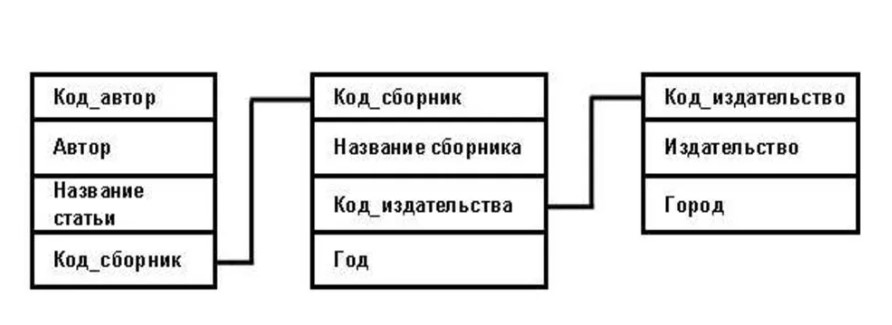
\includegraphics[scale=0.4]{3.png}}
	\caption{Страницы авторизации и регистрации}
	\label{fig:image}
\end{figure}





На рисунке 5 представлена страница карточки книги, находящихся в библиотеке. На ней есть возможность выбрать состояниие книги относительно пользователя:
\begin{itemize}
	\item хочу прочитать;
	\item в процессе;
	\item прочитано.
\end{itemize}

Также присутствует возможность сбросить состояние, удалить книгу и изменить местоположение книги в библиотеке. 

\begin{figure}[H]
	\center{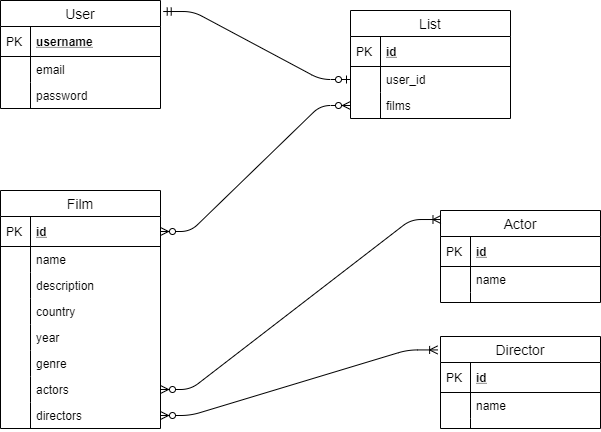
\includegraphics[scale=0.3]{4.png}}
	\caption{Страница карточки книги}
	\label{fig:image}
\end{figure}

На рисунке 6 показана страница реализации поиска по автору и/или названию.

\begin{figure}[H]
	\center{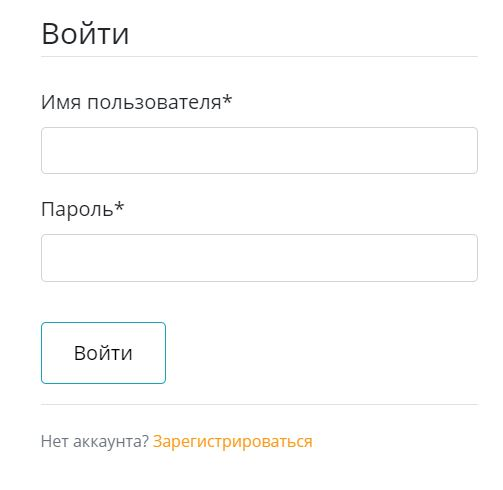
\includegraphics[scale=0.3]{5.png}}
	\caption{Страница поиска}
	\label{fig:image}
\end{figure}

Страница с формой добавления книги представлена на рисунке 7. 

\begin{figure}[H]
	\center{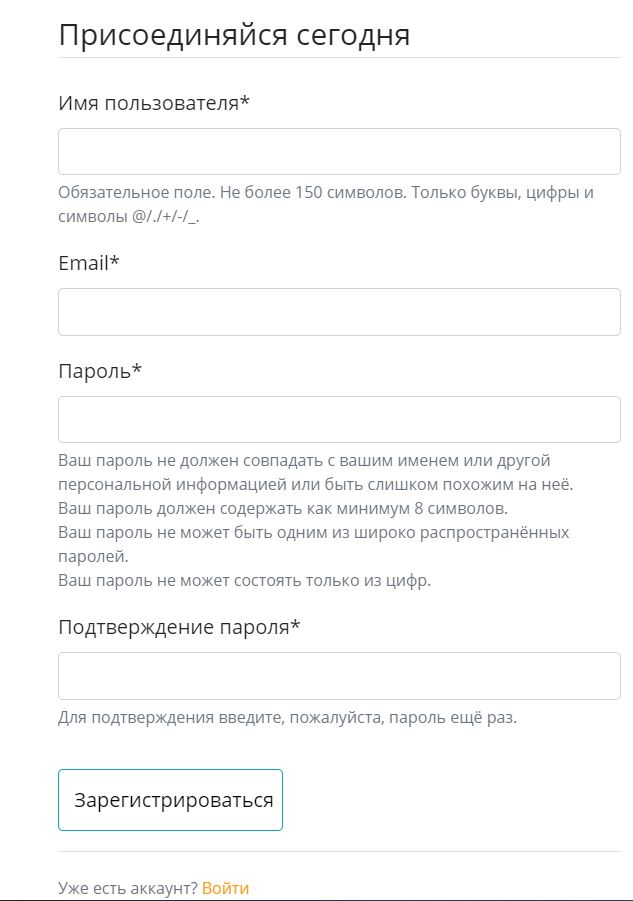
\includegraphics[scale=0.3]{6.png}}
	\caption{Страница добавления книги}
	\label{fig:image}
\end{figure}

В верхней части личного кабинета (рис. 8) пользователя расположена его личная информация  и количество книг, которые с ним связаны. В нижней части находится список этих книг. С этой страницы можно удалить связь с книгой, нажав на крестик в правом верхнем углу блока книги.

\begin{figure}[H]
	\center{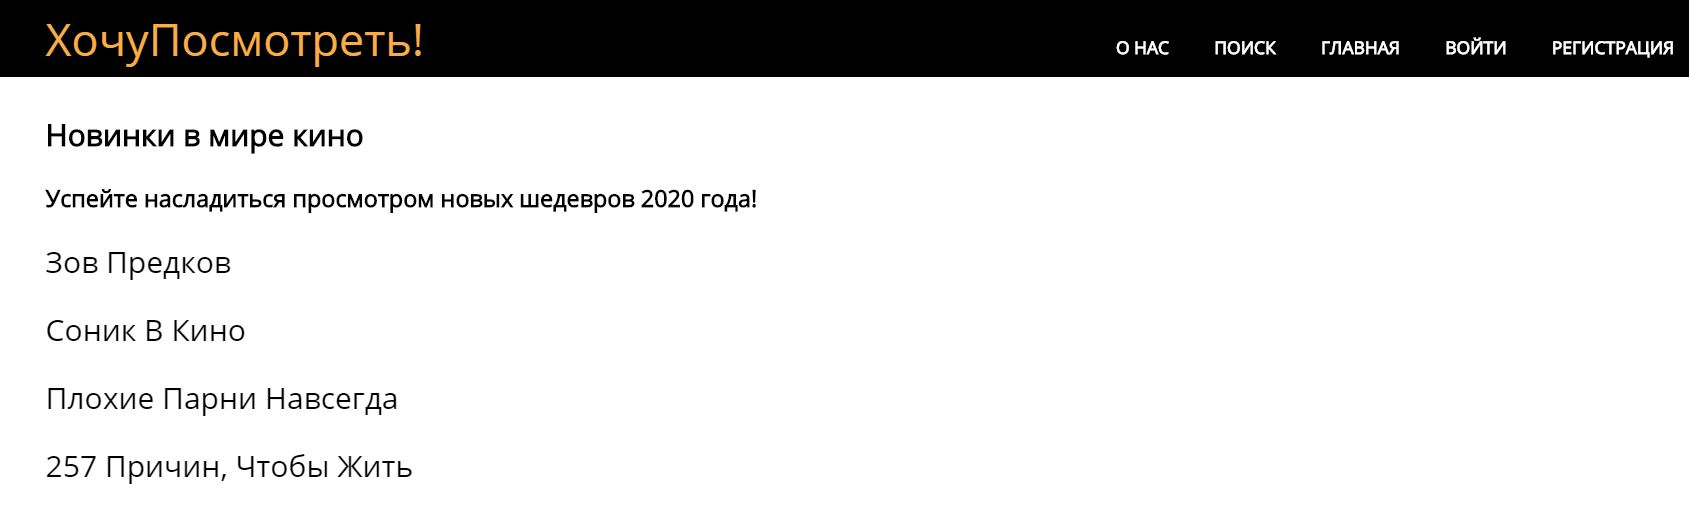
\includegraphics[scale=0.3]{7.png}}
	\caption{Личный кабинет}
	\label{fig:image}
\end{figure}

\newpage
\section*{Заключение}%
\addcontentsline{toc}{section}{Заключение}

В результате проделанной работы:
\begin{itemize}
	\item были продуманы функции, которые должно было решать приложение;
	\item проведен анализ инструментов, необходимых для проектирования и реализации задачи, в результате которого был выбраны такие инструменты, как SQLite, Flask;
	\item разработана структура базы данных, состоящая их нескольких сущностей;
	\item с помощью выбранных инструментов был реализован web-интерфейс, обладающий возможностью регистрировать пользователей, изменять состояние и местоположение книг, добавлять и удалять книги, а также осуществлять поиск по ключевым словам.
\end{itemize}
\end{document}